\documentclass[14pt ,a4paper]{extarticle}
\usepackage[top=1in , bottom=1in , left=0.5in , right=0.5in]{geometry}
\usepackage{graphicx}
\begin{document}
\tableofcontents
\pagebreak

\section{Fault And Its Classifications}
\begin{itemize}
    \item{Faults in electrical power systems are abnormal conditions that disrupt the normal flow of current. These disruptions can range from minor disturbances to catastrophic failures.}
    \item{Faults in electrical power systems can cause significant disruptions,
 including power outages, equipment damage, and safety hazards.}
\item{ To mitigate these effects, power system operators employ various protection measures such as protective relays, circuit breakers, and grounding systems.}
    \item{There are primarily open and short circuit faults}
    \item{Faults can be located using terminal fault location methods or cable screening methods}

    \item{Open Circuit fault occurs in the series of transmission line - Open Conductor Fault , 2 open conductor fault , 3 open conductor fault which causes excessive current to flow into the system}
    \item{They can be tolerated but if higher power then insulation breaks down and short circuit fault occurs}
    \item{Short Circuit Fault occurs due to insulation failure between a phase conductors and ground}
    \item{These includes}
        \begin{enumerate}
            \item{Symmetrical Faults}
            \item{Unsymmetrical Faults}
        \end{enumerate}
        \vspace{40pt}
    \subsection{Symmetrical Faults}
    \item{Arcing due to faults can lead to fire}
    \item{Voltage can fall below permissible value}
        \vspace{50pt}
        \item{Symmetrical Faults involves all three phases like}

        \begin{enumerate}
            \item{L-L-L}
            \item{L-L-L-G}
        \end{enumerate}
        \begin{center}
                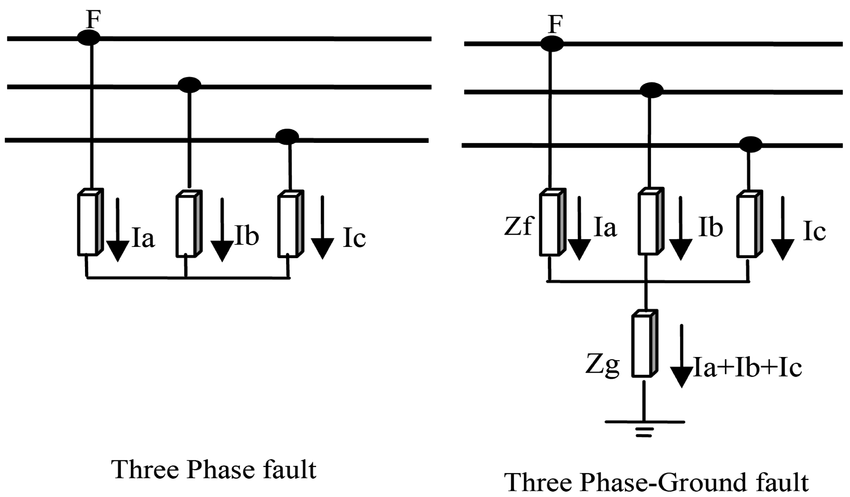
\includegraphics[width=0.6\textwidth]{./assets/Two-most-common-symmetrical-fault-types.png}
            \end{center}    
    \item{Majority of symmetrical faults occur at generator terminals , system stays balance but electrical equipments can get severly damaged}
    \item{They are the most severe type of fault with highest fault current but they happens rarely}
        \subsection{Unsymmetrical Faults}
    
    \item{These fault causes unsymmetrical current , meaning variation in phase and magnitude throughout all three phases }

    \item{These faults are more frequent faults }
    \item{These includes}
        \begin{enumerate}
            
            \item{L-G} 
            \item{L-L} 
            \item{L-L-G} 
            
        \end{enumerate}
        \begin{center}
                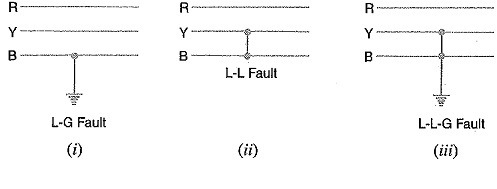
\includegraphics[width=0.6\textwidth]{./assets/Unsymmetrical-Faults-on-Three-Power-System.jpg}
            \end{center}    
    \item{In these faults conductors make contact with other conductor or with the ground or both}
    \item{L-L faults occurs mainly due to 2 lines swinging because of high speed winds}
    \item{Here the system is unbalanced because impedance level in each phase differs , causing unbalanced current to flow between the phases}
        
\end{itemize}
\section{ML Application in Fault Analysis}
\begin{itemize}
    \item{Machine Learning (ML) algorithms can be incredibly effective at identifying abnormal patterns in sensor data, which can signal potential faults or anomalies within a system.A technique by the name of Anomaly Detection can be used here.}
    \item{Techniques like Recurrent Neural Networks (RNNs) can analyze time-series data from sensors to detect faults based on temporal dependencies(severity of a fault is dependent on its relationship with other faults.}
    \item{We can use Supervised learning(with the help of labelled dataset) to classify faults into short circuit and open circuit faults}
    \item{ML models can be used to predict faults and do timely maintenance of the system using past data}
    \item{Specific location of faults can be identified with the help of ML models which can significantly reduce clearing time of the system  }
    \item{Convolution Neural Networks(CNNs) can be trained on fault signatures (waveforms ,phasors ) to classify faults  }
\end{itemize}

\section{ Research Papers }

\subsection{Integrating discrete wavelet transform with neural networks and machine
learning for fault detection in microgrids}

\begin{itemize}
    \item{Additional difficulties in microgrid fault detection due to distributed generation specifically the bidirectional flow of energy} 
    \item{conventional systems are ineffective due to low value of fault current in MG}
    \item{Techniques of protection differs on whether the MG is connects to main grid or is working in isolation mode}
    \item{It involves generator of different capacities and types of fault current producd at various levels}
    \item{DWT extracts wavelet coefficients}

\end{itemize}
\end{document}
